\clearpage 
\onecolumn
\appendix

\section{Experimental Setups}
\label{sec:experimental-setups}

This appendix documents the experimental setups used throughout this work. The figures are organized as follows:

\begin{itemize}
  \item Figures \ref{fig:cam1} and \ref{fig:cam2} show the initial camera setup used to visualize and validate speckle patterns.
  \item Figure \ref{fig:detectors} presents the different detectors used for alignment and baseline measurements.
  \item Figure \ref{fig:speckles} demonstrates how speckle patterns vary with different laser configurations.
  \item Figure \ref{fig:setup} shows the final experimental setup with the piezo disc.
  \item Figure \ref{fig:lasers} documents the various laser configurations developed during this work.
  \item Figure \ref{fig:config} visualises the speckle pattern for each laser configuration used.
\end{itemize}

\begin{figure}[t]
\centering
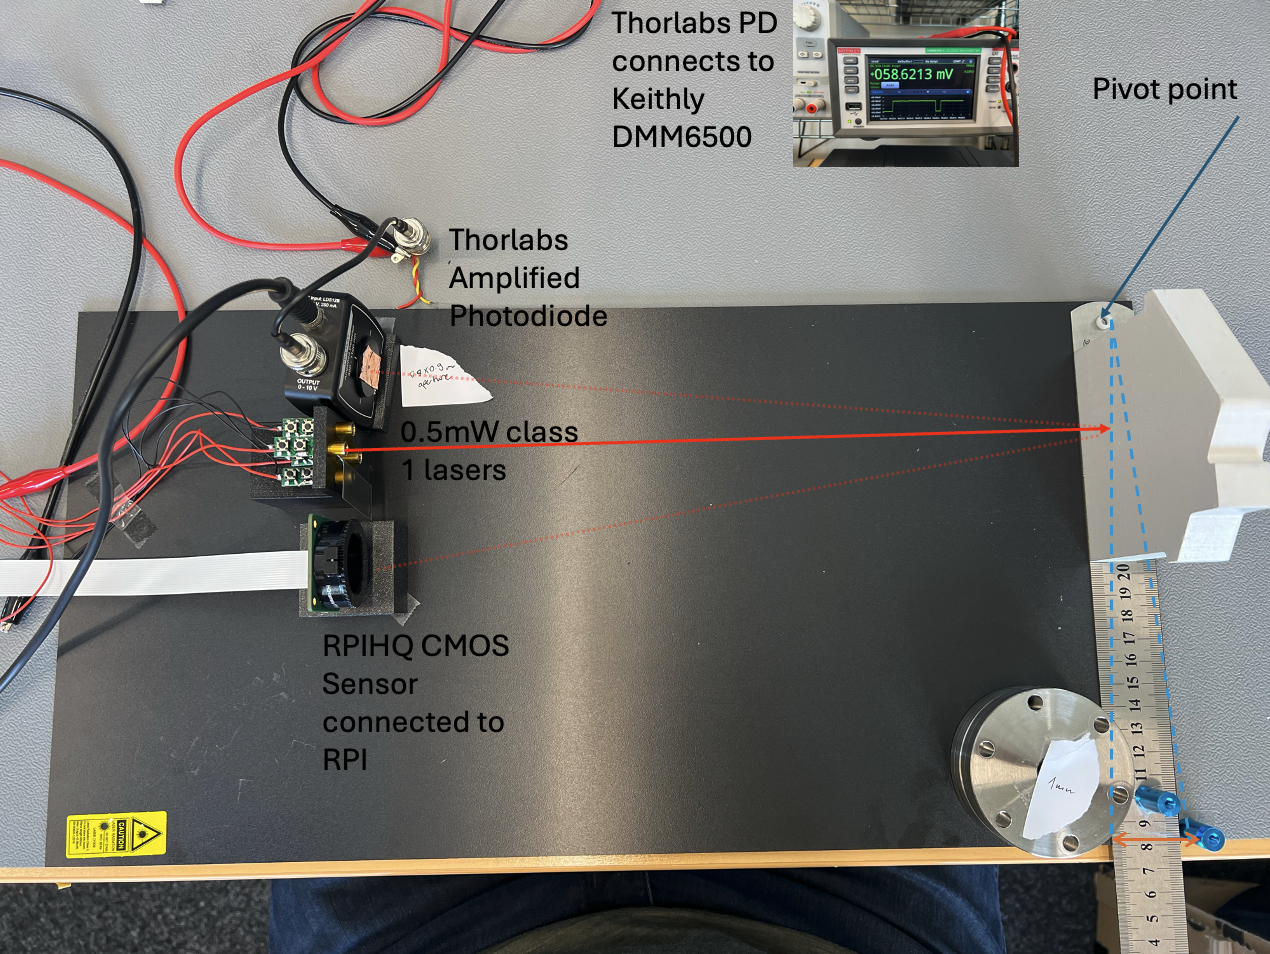
\includegraphics[width=\textwidth]{figures/impl/camera_setup.png}
\caption{A laser is pointed at a painted wooden surface. A multimeter measured the current from a masked photodiode. 
A RPI HQ camera is used as a reference to visualise the speckle pattern.}
\label{fig:cam1}
\end{figure}

\begin{figure}[t]
\centering
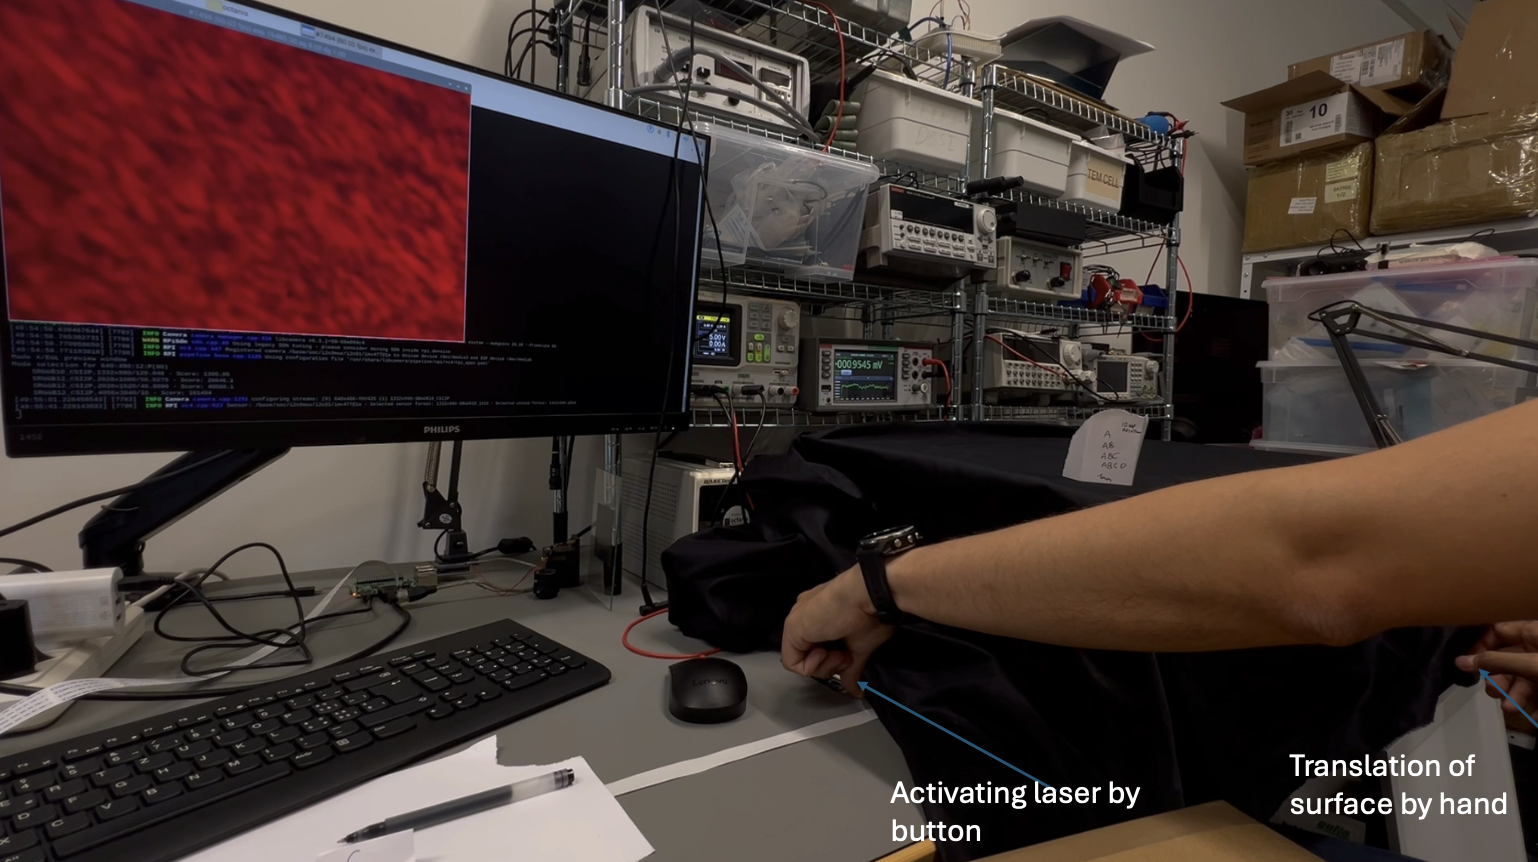
\includegraphics[width=\textwidth]{figures/impl/camera_setup2.png}
\caption{Speckle pattern visualised by RPI Cam HQ (from Setup in Figure \ref{fig:cam1})}
\label{fig:cam2}
\end{figure}

\begin{figure}[t]
\centering
\includegraphics[width=\widthnarrow]{figures/eval/detectors.png}
\caption{The Raspberry Pi No-IR (top left) was used to align invisible IR lasers, the Raspberry Pi HQ camera for 
showing speckle patterns and the (masked) Thorlabs detector for establishing a photocurrent baseline for our amplifier.}
\label{fig:detectors}
\end{figure}

\begin{figure*}[t]
\centering
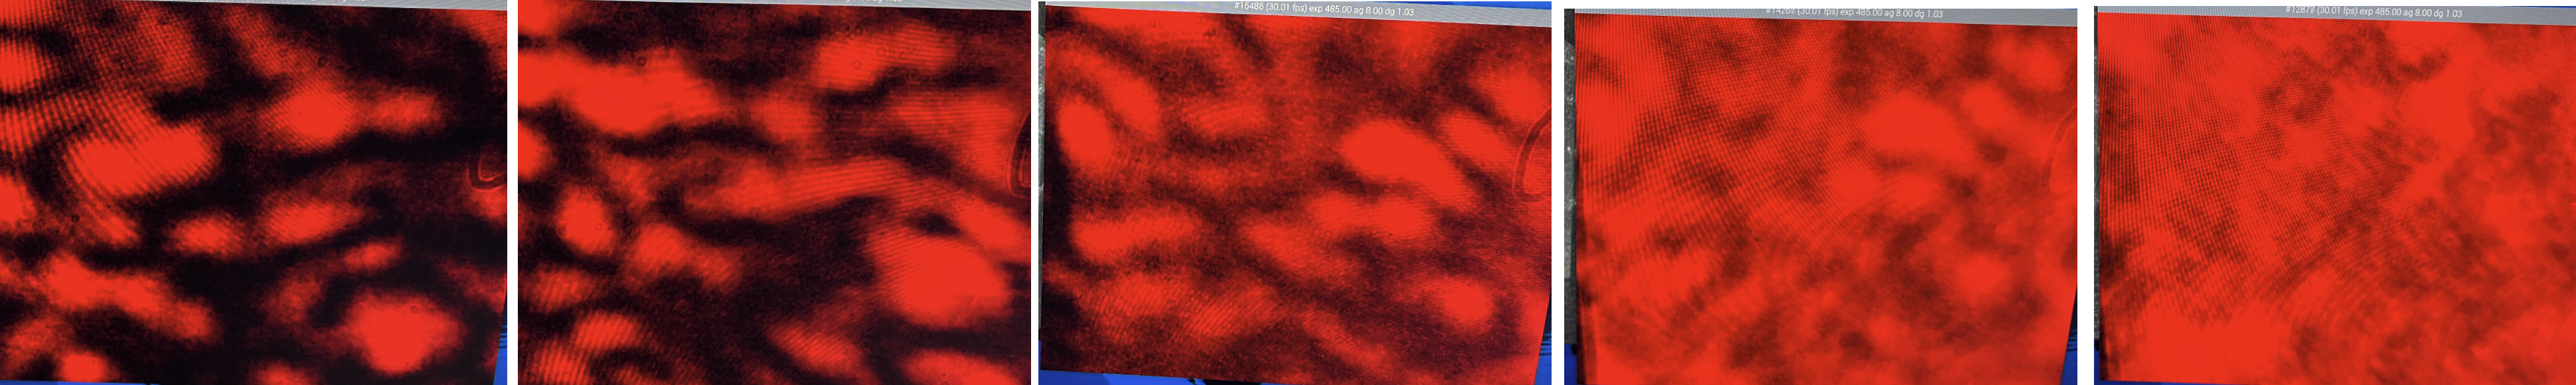
\includegraphics[width=\textwidth]{figures/eval/speckles}
\caption{Visualization of speckle patterns under different 1~mW IR laser configurations using the square 
laser array from Figure~\ref{fig:lasers}. Top left: 1 laser. Bottom right: 10 lasers.}
\label{fig:speckles}
\end{figure*}

\begin{figure*}[t]
\centering
\includegraphics[width=\textwidth]{figures/eval/typical_setup.png}
\caption{Photo of the experimental configuration with the piezo disc.}
\label{fig:setup}
\end{figure*}

\begin{figure*}[t]
\centering
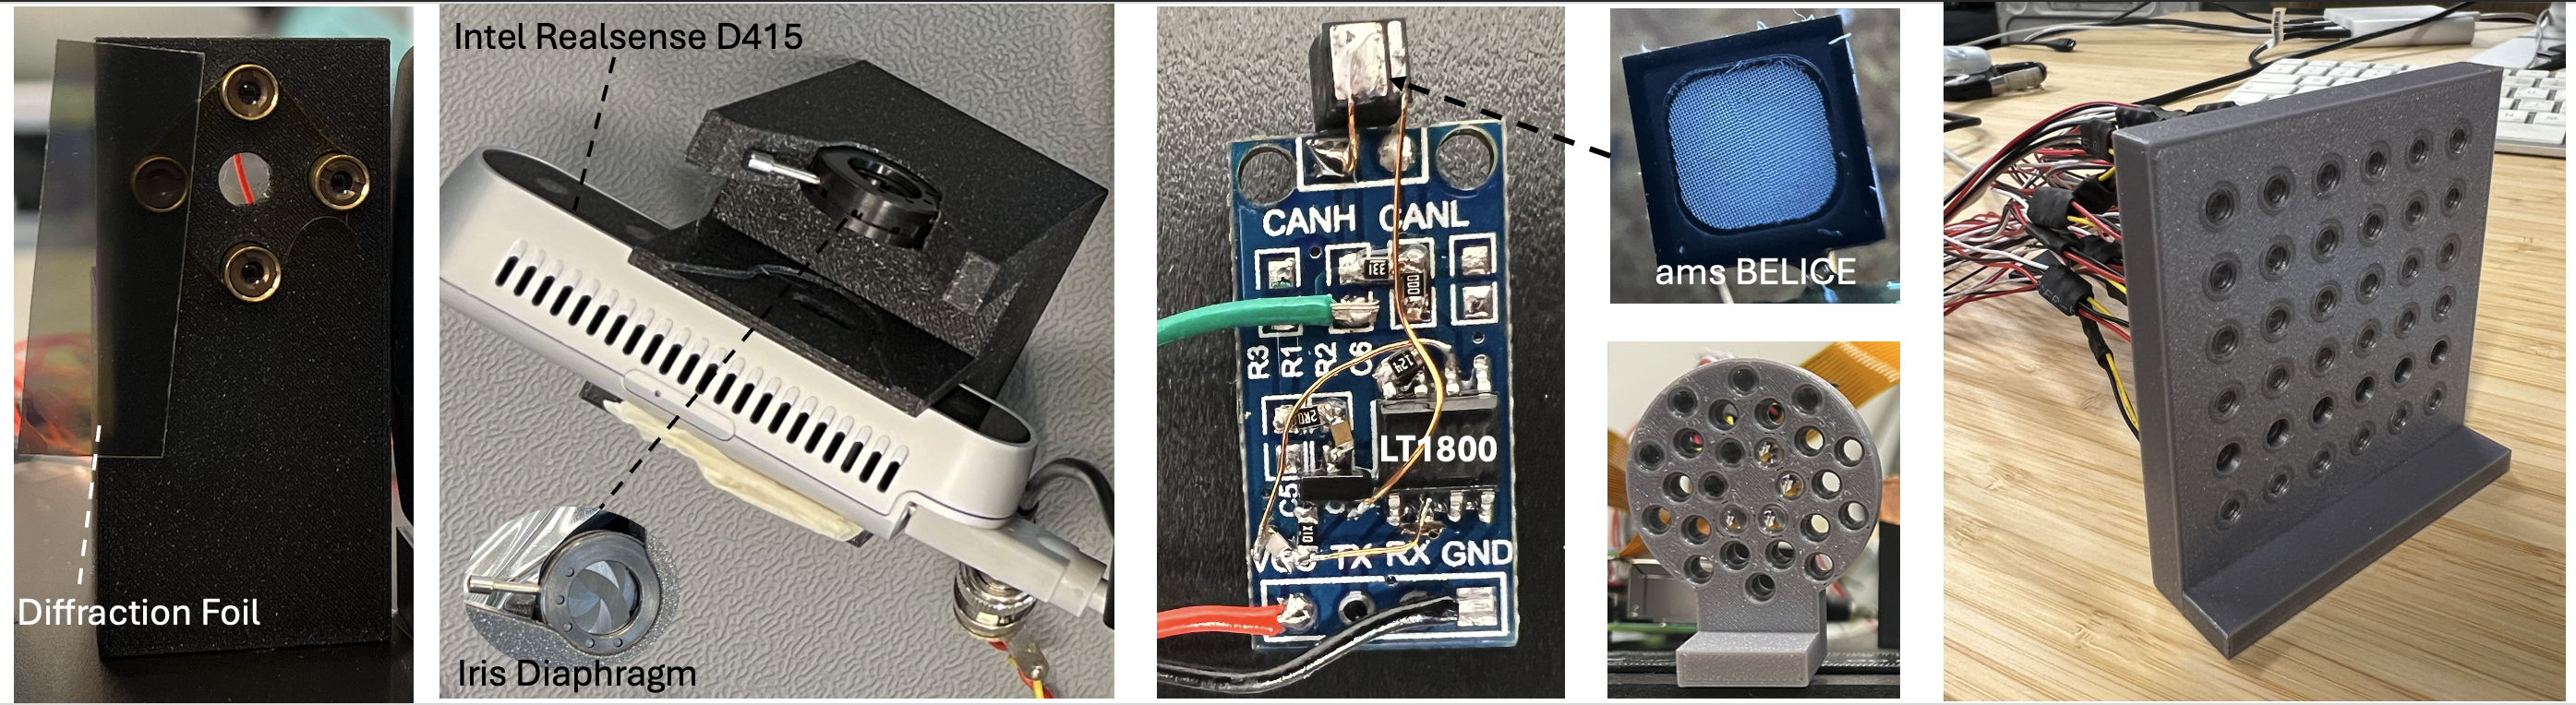
\includegraphics[width=\textwidth]{figures/eval/lasers}
\caption{The different laser setups used from left to right: Red laser for initial emulation experiments, 
Realsense 415 dot projector with iris, reverse engineered Realsense dot projector and driver circuit, 
discrete circular and square IR laser arrays.}
\label{fig:lasers}
\end{figure*}

    

\begin{figure*}[t]
\centering
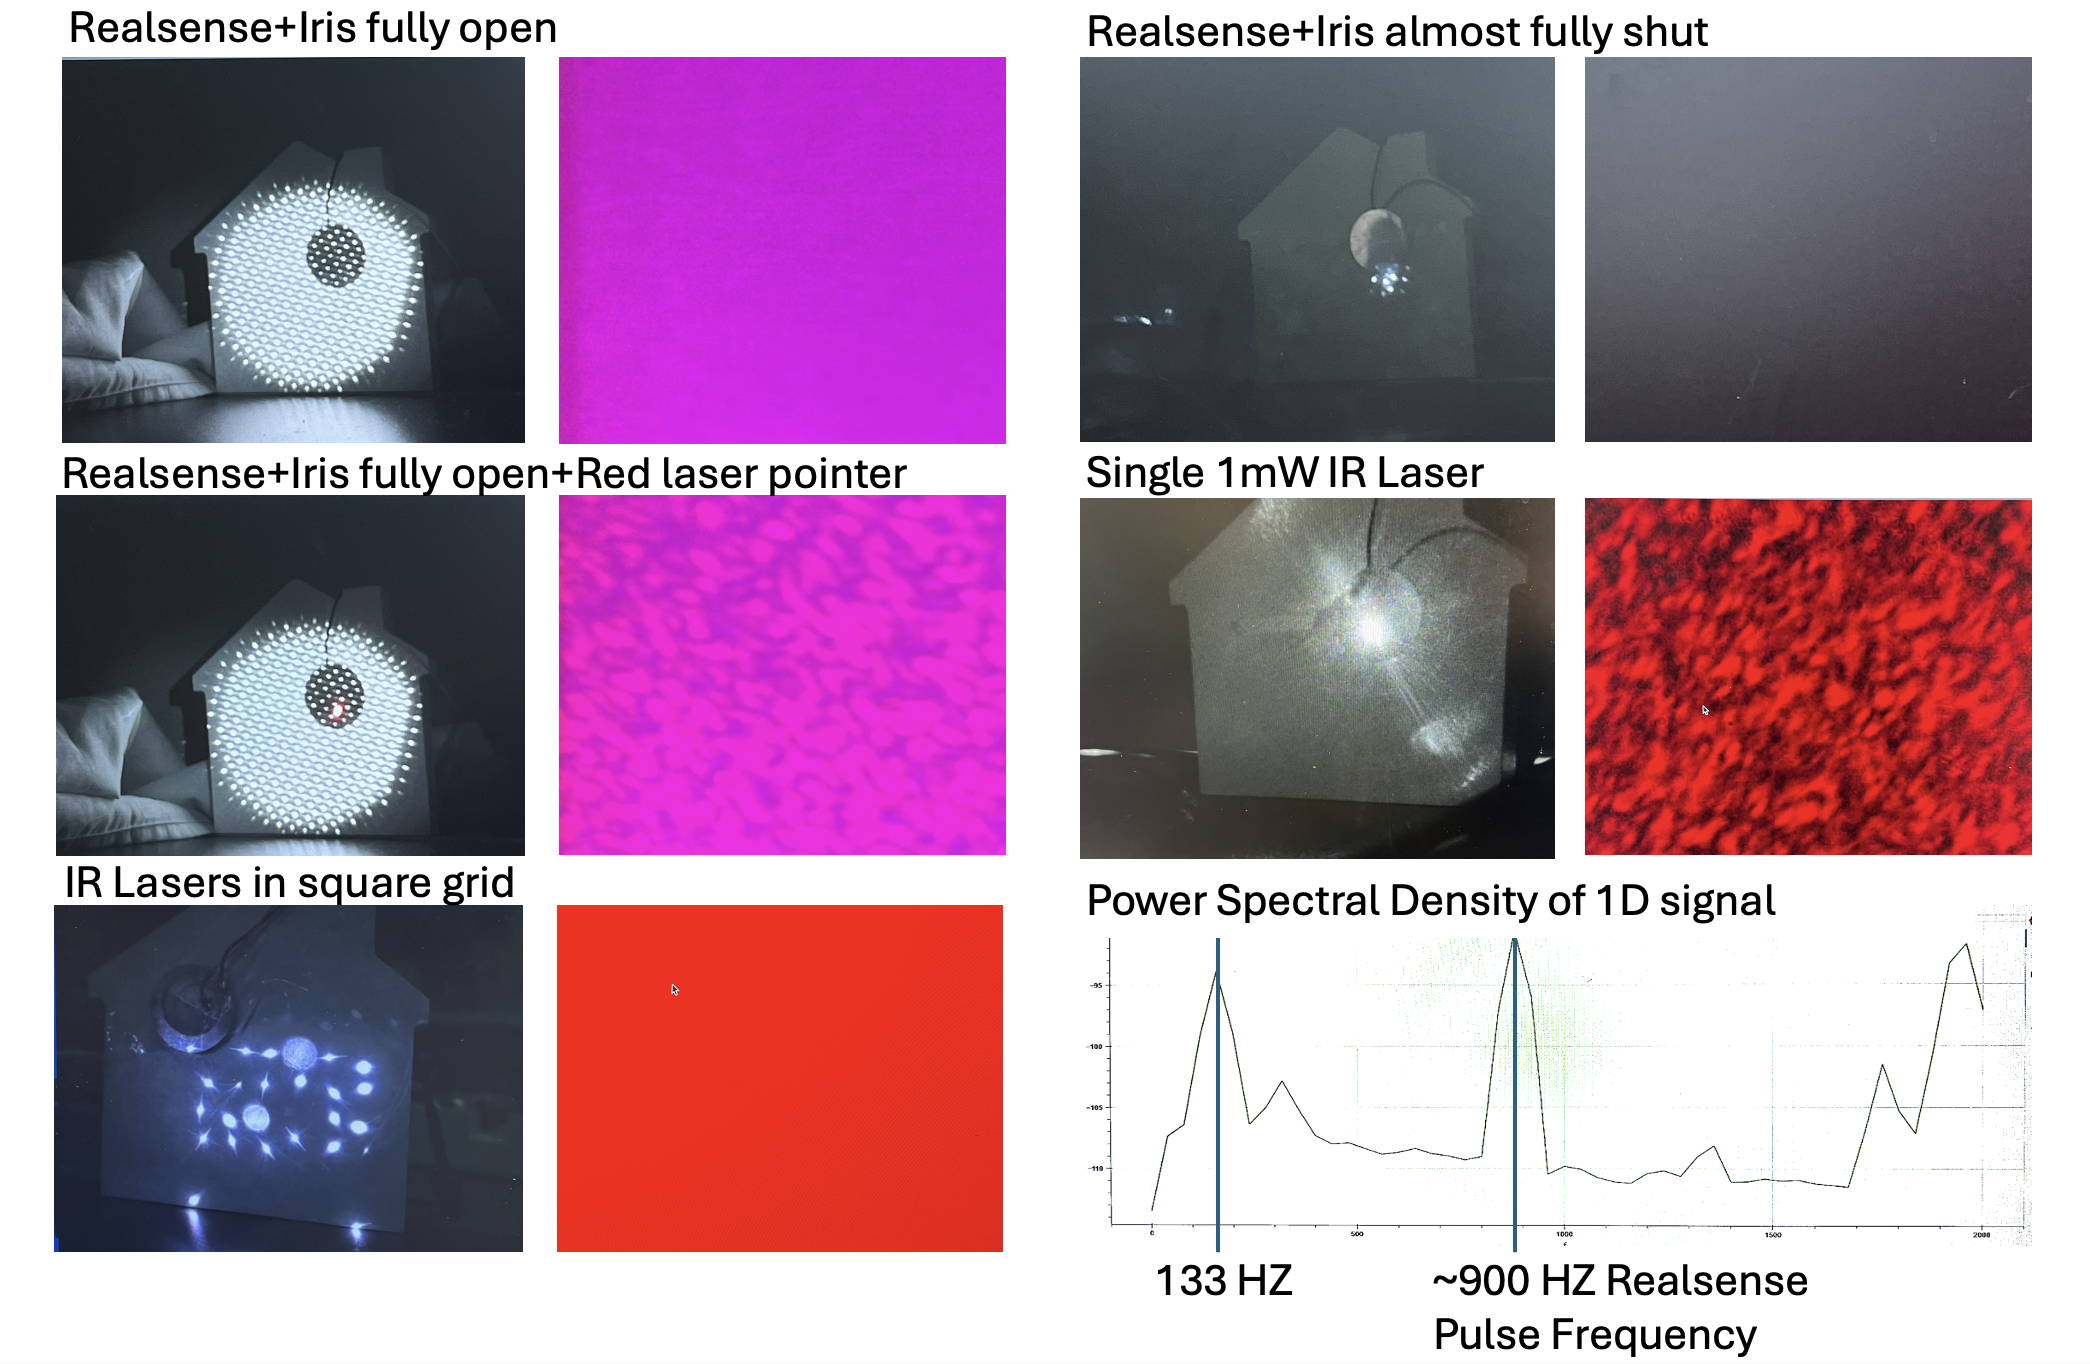
\includegraphics[width=\textwidth]{figures/results/configs}
\caption{Laser configuration and resulting speckle patterns on the camera sensor. Bottom right shows the PSD of the 1d signal. When the Realsense is used, we see a peak at 900 Hz due to the pulsing nature of the dot projector. Note that our detector can only pick up the Realsense speckle pattern if and only if the surface has high reflectivity and is aligned perfectly. The square grid lasers are somewhat distorted, due to mechanical stress on the low grade plastic collimating lenses used.}
\label{fig:config}
\end{figure*}

\begin{figure*}[t]
\centering
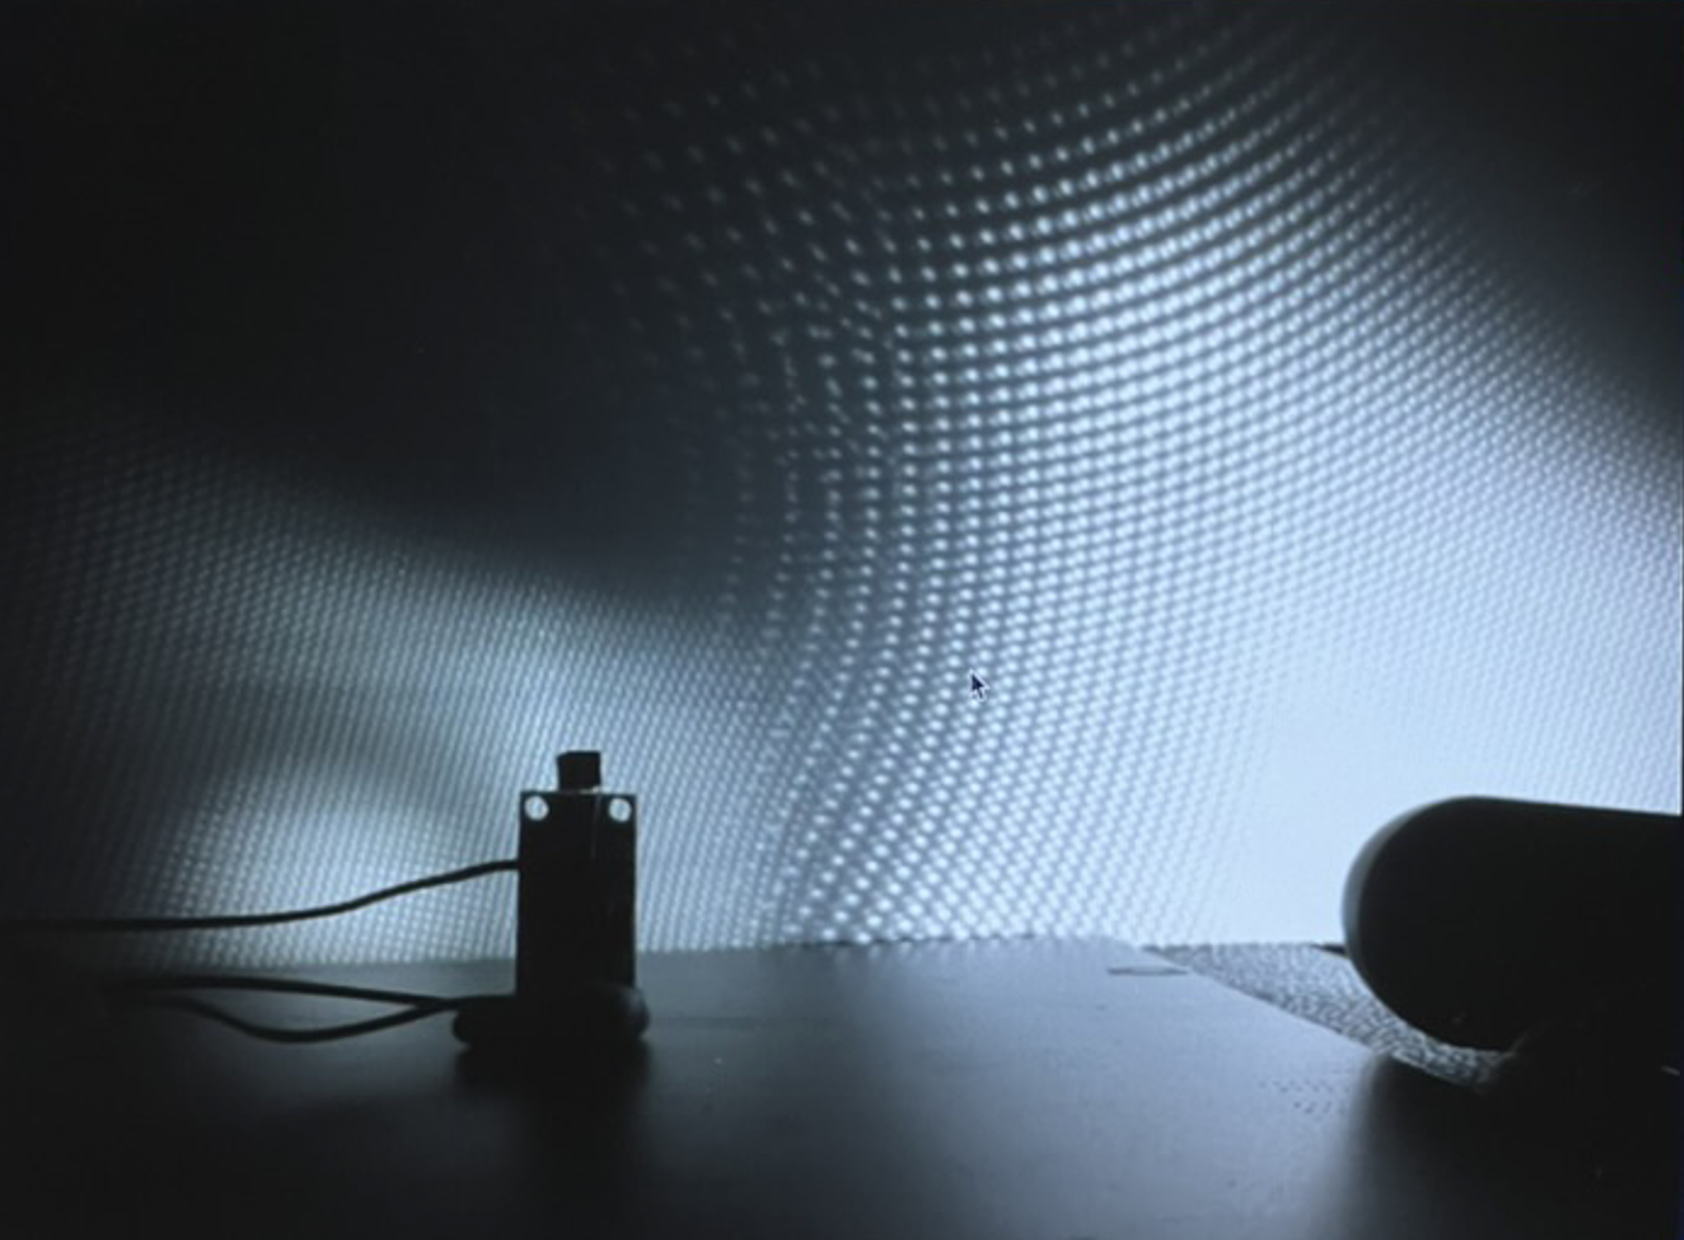
\includegraphics[width=\textwidth]{figures/results/rsvsdiy}
\caption{Our dot  project vs the Realsense camera. The pattern seams different, but this is due to the Realsense using 2 side by side dot projectors. If we cover up one, we get an identical pattern.}
\label{fig:rsvsdiy}
\end{figure*}
    
\onecolumn 